% Paper V: Fractional Memory for Frozen Language Models
% Ramiro Fontes, Quijotic Research LLC

\documentclass[11pt]{article}
\usepackage[margin=1in]{geometry}
\usepackage{amsmath,amssymb,amsthm,mathtools}
\usepackage{enumitem}
\usepackage{hyperref}
\usepackage{cleveref}
\usepackage{booktabs}
\usepackage{tikz}
\usepackage{pgfplots}
\pgfplotsset{compat=1.17}

\theoremstyle{plain}
\newtheorem{theorem}{Theorem}[section]
\newtheorem{proposition}[theorem]{Proposition}
\newtheorem{lemma}[theorem]{Lemma}

\theoremstyle{definition}
\newtheorem{definition}[theorem]{Definition}
\newtheorem{remark}[theorem]{Remark}

\newcommand{\E}{\mathbb{E}}
\newcommand{\Id}{\mathrm{Id}}

\title{Fractional Memory for Frozen Language Models:\\
  Architecture, Kernel, and When Each Matters}
\author{Ramiro Fontes\\
  Quijotic Research\\
  \texttt{ramirofontes@gmail.com}}
\date{\today}

\begin{document}
\maketitle

\begin{abstract}
A frozen language model augmented with a persistent
memory store can adapt to new information in real time.
We develop such a system and characterize the
contributions of its two main design choices: a
three-layer retrieval pipeline (canonical-form
\emph{normalize}, keyword-based \emph{route},
kernel-weighted \emph{rerank}) and the temporal
kernel that weights entries by age.

The architecture avoids a structural tradeoff that
both natural baselines face: overwriting policies
(\emph{keep-latest}) maximize current-state
accuracy by deleting superseded facts and then
score zero on historical queries by construction;
retaining policies (\emph{vanilla RAG}) preserve
history but cannot separate current from historical
values among content-similar updates and score
poorly on current-state queries.  The three-layer
kernel-weighted architecture reaches the
upper-right quadrant that neither baseline can
occupy: $82$--$83\%$ current-state accuracy with
$66$--$73\%$ historical-query accuracy, by
decoupling storage (retain everything) from
scoring (weight by age relative to the query's
reference time).

Architecture is the larger effect.  Against
vanilla retrieval-augmented generation on a
biographical benchmark, the three-layer system gains
$+27$~pp overall, with fact normalization alone
responsible for most of the gain.  This contribution
is robust across kernel choices.

Kernel choice matters in a second, more subtle way.
Mittag-Leffler's kernel
$E_\alpha(-\lambda\,\Delta t^\alpha)$, where
$\Delta t$ is the age of the entry and $\alpha, \lambda$
are kernel parameters, is the resolvent
of a fractional stochastic PDE and has a power-law tail
that an exponential kernel cannot match.  We prove and
demonstrate that for the exponential kernel
$e^{-\lambda t}$ the maximum age $\tau^*$ at which a
correct entry still outranks a moderately-scored
distractor is the fixed constant
$\tau^*_{\mathrm{exp}} = 1 + \lambda^{-1}\ln(r_c/r_d)$,
linear in $\lambda^{-1}$; for the Mittag-Leffler kernel
with $\alpha \in (0, 1)$, the analogous boundary
$\tau^*_{\mathrm{frac}}(\alpha, \lambda)$ grows
polynomially in $\lambda^{-1}$ with exponent $1/\alpha
> 1$ and can be made arbitrarily large by taking
$\alpha$ close to $0$.  Both retention boundaries are
independent of the deployment horizon; the structural
advantage is a super-polynomial gap in kernel-parameter
scaling, not a horizon-scaling claim.
Empirically, this structural property survives a
synthetic parameter-surface ablation, a dense EWMA audit,
a real-embedding MiniLM audit, and a matched-scale
calibration test over horizons, candidate-pool sizes,
update-rate regimes, and kernel families.  In the
synthetic best-tuned comparison the
fractional/Mittag-Leffler kernel attains mean accuracy
$0.572$, compared with $0.495$ for a dense $100$-point
EWMA audit, $0.458$ for a generic power-law family, and
$0.460$ for the best finite mixture of exponentials; in
the MiniLM surface it attains $0.706$, compared with
$0.661$ for dense EWMA and finite exponential mixtures
and $0.646$ for power-law.  The advantage is not merely
a longer-memory artifact: when EWMA and power-law
controls are matched to the fractional kernel's half-life
or finite-horizon effective memory, the best matched
control reaches only $0.585$ on the full MiniLM surface.
A structured local-decoder check with a fixed Ollama
model then shows that the improved memory selection
translates into answer accuracy in a frozen-decoder
adapter setting: fractional context selection reaches
$0.970\pm0.017$ versus $0.778\pm0.048$ for dense EWMA
and $0.950\pm0.024$ for power-law.  The same ablations
also identify the limitation: the fractional kernel is
not the uniformly most robust family under arbitrary
mistuning, and at long horizons candidate recall becomes
the bottleneck.  Thus the empirical contribution is not
merely ``fractional beats exponential''; it is that the
fractional resolvent gives the best tuned temporal
reranking when the correct fact survives routing, while
retrieval quality still caps end-to-end performance.

We report several experimental findings and characterize
two regimes in which the kernel's effect is small: a
uniform-rate short-horizon regime where any monotone
temporal weighting suffices, and a long-horizon regime
where candidate-pool signal-to-noise ratio dominates.

Deployment is live.  Updates arrive in real time at
$O(1)$ per entry, and no weights are modified.
\end{abstract}


\section{Introduction}\label{sec:intro}

Frozen language models cannot update what they know.
Retraining or fine-tuning is one response; retrieval
augmentation is another.  When retrieval is the
answer, the memory store becomes the place where
temporal structure must live: what was true yesterday
should not overwrite what is true today, and what was
true ten years ago should not vanish just because it
is ten years ago.

A standard retrieval-augmented generation system treats
all entries uniformly: cosine similarity to a query
retrieves a shortlist, and a generation model produces
an answer.  This fails on temporal reasoning in two
ways.  First, when multiple updates to the same
attribute have similar embeddings (``Alex's salary is
\$240{,}000,'' ``Alex's salary is \$380{,}000''), the
retrieval cannot distinguish current from historical
values.  Second, when queries are temporal
(``What was Alex's employer when Luna was
adopted?''), cosine similarity alone has no mechanism
for resolving ``when Luna was adopted'' to a
timestamp and using it as a lens.

We study a system that addresses both: a three-layer
architecture (\emph{normalize}, \emph{route},
\emph{rerank}) that wraps a kernel-weighted memory
store around a frozen language model.  The contribution
of this paper is empirical: we report several experiments
isolating what each component buys, and characterize
the regimes where the contribution is large versus
small.

The central results are:

\begin{enumerate}[label=\textbf{(\arabic*)}]
\item \textbf{The three-layer architecture produces a
  $+27$~pp gain over vanilla RAG} on the static
  biographical benchmark, with fact normalization
  alone responsible for most of the gain
  (\Cref{sec:static}).  The architecture's contribution
  is robust across kernel choices.

\item \textbf{The Mittag-Leffler kernel has a
  structural retention property that no exponential
  kernel can match} (\Cref{sec:structural}): the
  maximum age $\tau^*$ at which the kernel
  preserves an old-but-correct entry against a fresh,
  moderately-scored distractor is a fixed constant
  that depends on kernel parameters but not on the
  retrieval horizon.  For exponential kernels
  $\tau^*_{\mathrm{exp}} = 1 + \lambda^{-1}
  \ln(r_c/r_d)$ is linear in $\lambda^{-1}$.  For
  Mittag-Leffler kernels with $\alpha \in (0, 1)$,
  $\tau^*_{\mathrm{frac}}$ grows polynomially in
  $\lambda^{-1}$ with exponent $1/\alpha > 1$, and
  is unbounded in the limit $\alpha \to 0$.  At the
  tuning $\lambda = 0.05$ used in
  \Cref{fig:retention}: EWMA retention is fixed at
  $32$ months regardless of horizon;
  Mittag-Leffler at $\alpha = 0.3$ saturates at
  $\approx 880$ months; at $\alpha = 0.2$ the
  retention boundary exceeds $30{,}000$ months and
  the kernel tracks $\min(T, \tau^*) = T$ at every
  horizon tested ($120, 480, 1200, 2400$ months).


\item \textbf{This structural property survives a
  parameter-surface ablation} across horizons
  $60,120,480,1200$, candidate-pool sizes
  $K\in\{10,25,50,100,250\}$, uniform and mixed update
  regimes, and several temporal-kernel families
  (\Cref{sec:empirical}).  The best-tuned
  fractional/Mittag-Leffler family attains aggregate
  accuracy $0.572$, versus $0.495$ for a dense EWMA
  audit, $0.458$ for a generic power-law family, and
  $0.460$ for the best finite exponential mixture.

\item \textbf{Two regimes where the kernel's effect
  is small.}  At uniform attribute rates with tuned
  parameters and ample candidate recall, monotone
  long-memory kernels can tie.  At extended horizons
  or large stores, the candidate pool degrades and
  the kernel's advantage shrinks because the correct
  fact is no longer routed into the top-$K$ set
  (\Cref{sec:when_kernel_secondary}).

\item \textbf{The system achieves live adaptation at
  $O(1)$ cost per entry} (\Cref{sec:deployment}):
  $0\% \to 79.3\%$ on current-state queries across
  twenty real-time updates, without any weight
  modification.  A historical-state capability
  (\emph{temporal lens}) scores $100\%$ versus
  $41.7\%$ for standard retrieval.

\item \textbf{The architecture reaches a
  (current-state, historical-query) accuracy region
  that the natural baselines cannot occupy by
  design} (\Cref{sec:pareto}).  Overwriting
  policies score zero on historical queries;
  retention policies score poorly on current-state
  queries against content-similar updates.  The
  three-layer architecture achieves $82$--$83\%$
  current-state with $66$--$73\%$ historical in
  the same run.
\end{enumerate}

Structural property and system-level gain are
separate results.  One is a theorem-like finding about
kernel asymptotics; the other is an empirical
statement about a specific benchmark in a specific
regime.  Both are true.  Neither implies the other.

\paragraph{Theoretical backing.}  The kernel is not
chosen ad hoc.  It is the resolvent of the fractional
stochastic PDE
$\partial_t^\alpha m = -\lambda m + \mathrm{noise}$,
where $\partial_t^\alpha$ is the Caputo fractional
derivative.  The connection between this kernel and
the operator factorization
$(\Id - \E)F = \delta\,\Pi\,DF$ is developed in
\cite{fontes2026opfac,fontes2026fracmem}; the present
paper is the applied half of that development and
does not depend on the theoretical details.


\section{Retention at Scale}\label{sec:chart}

Before developing the system, we show the single
finding that distinguishes the fractional kernel from
any exponential kernel.  We construct a controlled
retention test: a correct fact at age $\tau$ with
relevance $0.75$ competes against a fresh
(age-$1$) distractor with relevance $0.55$.
For each kernel $w$ (the temporal weighting function
evaluated at age, formalized in \Cref{sec:architecture})
at each parameter setting,
the \emph{max retention age} is the largest $\tau$ at
which the correct fact's score
$r_\text{correct}\cdot w(\tau)$ exceeds the
distractor's score $r_\text{distract}\cdot w(1)$.
No randomness.  No candidate pool.  Pure kernel.

\begin{figure}[h]
\centering
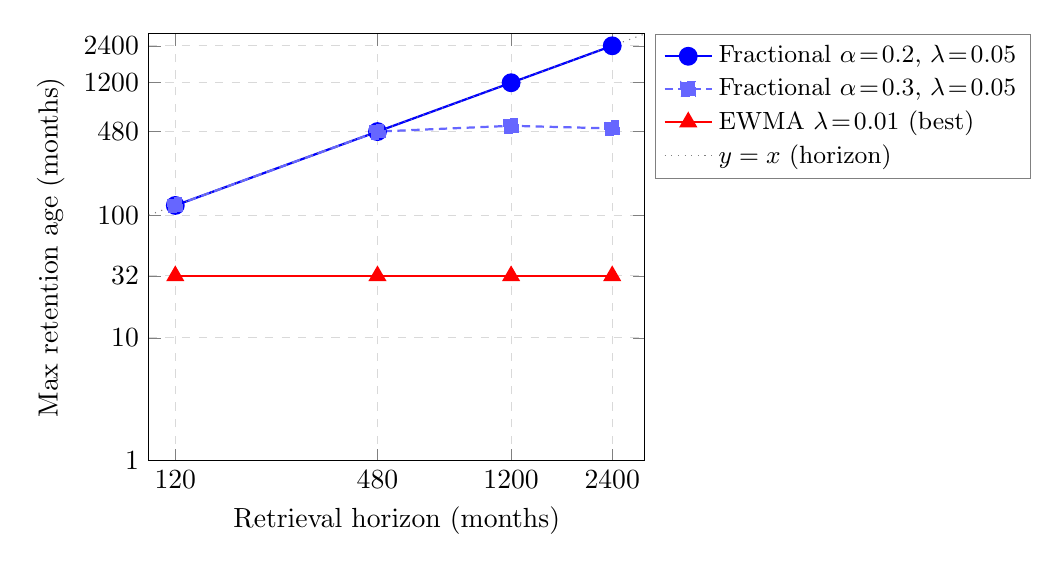
\begin{tikzpicture}
\begin{axis}[
    width=0.65\textwidth,
    height=7cm,
    xlabel={Retrieval horizon (months)},
    ylabel={Max retention age (months)},
    xmode=log,
    ymode=log,
    log basis x=10,
    log basis y=10,
    xmin=100, xmax=3000,
    ymin=1, ymax=3000,
    xtick={120, 480, 1200, 2400},
    xticklabels={120, 480, 1200, 2400},
    ytick={1, 10, 32, 100, 480, 1200, 2400},
    yticklabels={1, 10, 32, 100, 480, 1200, 2400},
    legend style={
        at={(1.02,1)}, anchor=north west,
        fill=white, draw=black!50,
        font=\small,
    },
    legend cell align={left},
    grid=major,
    grid style={dashed, gray!30},
]
% Fractional alpha=0.2, lambda=0.05: tau* exceeds every tested horizon
\addplot[thick, blue, mark=*, mark size=3pt] coordinates {
    (120, 120)
    (480, 480)
    (1200, 1200)
    (2400, 2400)
};
\addlegendentry{Fractional $\alpha\!=\!0.2$, $\lambda\!=\!0.05$}

% Fractional alpha=0.3, lambda=0.05: grows but saturates
\addplot[thick, blue!60, mark=square*, mark size=2.5pt, densely dashed] coordinates {
    (120, 120)
    (480, 480)
    (1200, 535)
    (2400, 509)
};
\addlegendentry{Fractional $\alpha\!=\!0.3$, $\lambda\!=\!0.05$}

% EWMA lambda=0.01: fixed at 32
\addplot[thick, red, mark=triangle*, mark size=3pt] coordinates {
    (120, 32)
    (480, 32)
    (1200, 32)
    (2400, 32)
};
\addlegendentry{EWMA $\lambda\!=\!0.01$ (best)}

% Diagonal reference line y=x
\addplot[dotted, black!50] coordinates {
    (100, 100)
    (3000, 3000)
};
\addlegendentry{$y = x$ (horizon)}

\end{axis}
\end{tikzpicture}
\caption{Max retention age versus retrieval horizon.
  A correct fact at age $\tau$ (relevance $0.75$)
  competes against a fresh distractor (age $1$,
  relevance $0.55$).  Each curve plots $A(T) =
  \min(T, \tau^*)$, where $\tau^*$ is the
  kernel-level retention boundary.  For the EWMA
  kernel $\tau^* = 32$ months: its curve is flat at
  the boundary regardless of horizon.  For
  Mittag-Leffler at $\alpha = 0.3$, $\tau^* \approx
  880$ months: the curve tracks the diagonal at
  short horizons and saturates as $T$ grows past
  $\tau^*$ (the empirical saturation points at
  $T = 1200, 2400$ are $535, 509$, close to the
  computed $\tau^*$). For Mittag-Leffler at $\alpha =
  0.2$, $\tau^* \approx 31{,}000$ months: the curve
  tracks $T$ at every horizon tested because no
  horizon reaches $\tau^*$.  The distinction
  \Cref{thm:retention} formalizes is in how $\tau^*$
  scales with the kernel's decay parameters: linear in
  $\lambda^{-1}$ for the exponential, polynomial in
  $\lambda^{-1}$ with exponent $1/\alpha > 1$ for the
  Mittag-Leffler kernel, and unbounded as
  $\alpha \to 0$.}
\label{fig:retention}
\end{figure}

Exponential retention is bounded by $O(\lambda^{-1})$.
Mittag-Leffler retention is bounded by $O(\lambda^{-1/\alpha})$
and can be made arbitrarily large by taking $\alpha$ small.
Both bounds are independent of the retrieval horizon; the
structural distinction is in how each scales with kernel
parameters.  What follows develops what this buys at the
system level, and what it does not.


\section{Architecture}\label{sec:architecture}

A fact store of $(entity, attribute, value, timestamp)$
tuples is queried by natural-language questions.  The
architecture routes each query through three layers.

\paragraph{Layer 1: Normalize.}  Incoming facts are
rewritten to a canonical template per category before
embedding.  ``Alex just got promoted to Senior
Engineer'' becomes the normalized form
\texttt{alex.title = senior\_engineer @ month 14}.
Normalization accomplishes two things.  First, it
aligns the embeddings of same-category facts, so that
two salary updates embed similarly and the retrieval
problem becomes temporal disambiguation rather than
content matching.  Second, it enables exact-match
routing (Layer 2).

Fact normalization is the single highest-impact
component.  On the static benchmark (\Cref{sec:static}),
normalization alone lifts location retrieval from
$0\%$ to $100\%$ and total accuracy by $+27$ points
over vanilla RAG.

\paragraph{Layer 2: Route.}  A keyword-based router
decides whether a query requires temporal reasoning.
Queries containing explicit temporal phrasing
(``current,'' ``latest,'' ``when,'' ``in month X'')
are routed to the temporal-reranking pipeline; others
are answered by cosine similarity alone.  The router
achieves $89\%$ recall on temporal queries and $100\%$
precision on static ones, preserving static accuracy
at $83.3\%$ while enabling temporal disambiguation
where needed.  A learned router would likely improve
coverage at the cost of latency.

\paragraph{Layer 3: Rerank.}  For temporal queries, a
cosine-similarity shortlist of the top-$K$ facts is
reranked by the combined score
$r \cdot w(|t_\text{query} - t_\text{fact}|)$,
where $r$ is the cosine similarity and $w$ is the
temporal kernel.  The argmax of the combined score is
the retrieved fact.  This separates content retrieval
(cosine) from temporal disambiguation (kernel); the
kernel acts as a tiebreaker within a candidate pool
that cosine has already narrowed.

\paragraph{Why three layers.}  Normalize without route
is lossy: it applies temporal weighting to static
queries where timestamps are irrelevant, degrading
accuracy on those queries.  Route without normalize
cannot create the temporal-ambiguity regime where
kernel weighting is useful.  Rerank without normalize
and route is equivalent to cosine with a temporal prior,
which neither resolves ambiguous same-category
embeddings nor preserves static accuracy.  The
experiments (\Cref{sec:static}) confirm that each
layer contributes something the others cannot.


\section{Static Benchmark}\label{sec:static}

\paragraph{Setup.}  A user named ``Alex'' is tracked
across $24$ months: salary changes ($5$ updates,
$\$240$k $\to \$420$k), job transitions ($4$ titles
at $3$ companies), relocations ($4$ cities), and $12$
other evolving attributes.  The store contains $121$
facts: $62$ with superseded earlier versions, $59$
static.  The benchmark is $87$ questions across $16$
categories, half temporal and half static.

\paragraph{Methods compared.}

\begin{itemize}[leftmargin=*]
\item \emph{Vanilla RAG.}  Cosine similarity over raw
  facts, top-$1$ retrieval.
\item \emph{Keep-latest.}  Vanilla RAG on a store
  that has deleted superseded versions.  A strong but
  destructive baseline.
\item \emph{Fractional (3-layer).}  Full architecture
  with the Mittag-Leffler kernel.
\end{itemize}

\paragraph{Results.}

\begin{center}
\begin{tabular}{@{}lrrrc@{}}
\toprule
Method & Temporal & Static & Overall & History? \\
 & ($n\!=\!57$) & ($n\!=\!30$) & ($n\!=\!87$) &
   retained \\
\midrule
Vanilla RAG & $19.3\%$ & $83.3\%$ & $41.4\%$
  & \checkmark \\
Keep-latest & $75.4\%$ & $86.7\%$ & $79.3\%$
  & $\times$ \\
\midrule
Fractional (3-layer) & $66.7\%$ & $83.3\%$ & $72.4\%$
  & \checkmark \\
\bottomrule
\end{tabular}
\end{center}

A $72.4\%$ overall is $+31$~pp over vanilla RAG.
Keep-latest scores higher ($79.3\%$) but does so by
deleting superseded facts---on queries that ask about
earlier states, it scores $0\%$ because the facts no
longer exist (see \Cref{sec:deployment}, mixed-query
benchmark).  A $7$-point gap between fractional and
keep-latest on the static benchmark is the cost of
retaining history.

\paragraph{Ablations.}  Removing each layer in turn
quantifies its contribution.  Fact normalization is
the largest single factor: without it, the location
category scores $0\%$ because the raw fact
embeddings of ``moved to Denver'' and ``relocated to
New York'' are nearly identical and no temporal
kernel can separate them.  Routing preserves static
accuracy at $83.3\%$; without it, applying the kernel
unconditionally degrades static queries by $\sim\!8$
points.  Reranking (rather than global kernel
scoring) prevents kernel weight from dominating
cosine in cross-category cases.


\section{Retention: A Structural Theorem}\label{sec:structural}

We now formalize the observation illustrated in
\Cref{fig:retention}: the maximum age at which a kernel
preserves a correct fact against a distractor is a fixed
constant that depends on kernel parameters, and this
constant scales very differently for the exponential
kernel versus the Mittag-Leffler kernel.

\subsection{Setup}

Fix relevance scores $r_c > r_d > 0$ for a correct
fact at age $\tau$ and a distractor at age $1$.  The
correct fact is retrieved when
$r_c \cdot w(\tau) > r_d \cdot w(1)$.  Since $w$ is
positive and strictly decreasing to $0$ for every
kernel we consider, the set of $\tau \geq 1$
satisfying this condition is an interval
$[1, \tau^*(w))$ for some finite
$\tau^*(w) \in [1, \infty)$.  Define the
\emph{retention boundary}
\[
\tau^*(w) \;=\; \max \big\{ \tau \geq 1
  : r_c\,w(\tau) > r_d\,w(1) \big\}.
\]
For any horizon $T \geq 1$, the \emph{max retention
age inside the horizon} is
\[
A(T) \;=\; \max \big\{ \tau \in \{1, \ldots, T\}
  : r_c\,w(\tau) > r_d\,w(1) \big\} \;=\; \min(T,
  \tau^*(w)).
\]
$A(T)$ is what \Cref{fig:retention} measures.  It is
pinned to the horizon when $T \leq \tau^*$ and flat at
$\tau^*$ once $T$ exceeds it.  The structural content
of the theorem is in $\tau^*$, not $A(T)$: both
kernels have a finite retention boundary, but the
boundaries scale differently with kernel parameters.

\begin{theorem}[Retention boundary scaling]
\label{thm:retention}
Let $w_{\mathrm{exp}}(t) = e^{-\lambda t}$,
$w_{\mathrm{frac}}(t) = E_\alpha(-\lambda t^\alpha)$
with $\alpha \in (0, 1)$, $\lambda > 0$, and
$w_{\mathrm{power}}(t) = (1+t)^{-\beta}$ with
$\beta > 0$.  Assume $r_c > r_d$.
\begin{enumerate}
\item \textnormal{(Exponential, linear in
  $\lambda^{-1}$.)}  The retention boundary of the
  exponential kernel is given exactly by
  \[
  \tau^*_{\mathrm{exp}}(\lambda)
  \;=\; 1 + \frac{1}{\lambda}\,
    \ln\!\frac{r_c}{r_d}.
  \]

\item \textnormal{(Mittag-Leffler, polynomial in
  $\lambda^{-1}$ with exponent $1/\alpha$.)}  For
  $\lambda$ small enough that
  $\tau^*_{\mathrm{frac}}(\alpha, \lambda)$ lies in
  the asymptotic regime of $E_\alpha$, the retention
  boundary satisfies
  \[
  \tau^*_{\mathrm{frac}}(\alpha, \lambda)
  \;=\; \Bigl(\frac{r_c}
    {r_d\,w_{\mathrm{frac}}(1)\,\lambda\,
    \Gamma(1-\alpha)}\Bigr)^{1/\alpha}
    \,(1 + o(1)),
  \]
  so $\tau^*_{\mathrm{frac}}$ grows as
  $\lambda^{-1/\alpha}$ for fixed $\alpha$, and
  $\tau^*_{\mathrm{frac}}(\alpha, \lambda) \to
  \infty$ as $\alpha \to 0$ for any fixed $\lambda$.

\item \textnormal{(Power-law, exponential in
  $\beta^{-1}$.)}  The retention boundary of the
  power-law kernel is given exactly by
  \[
  \tau^*_{\mathrm{power}}(\beta)
  \;=\; 2\,\Bigl(\frac{r_c}{r_d}\Bigr)^{1/\beta}
    - 1.
  \]
  In particular, $\tau^*_{\mathrm{power}}(\beta) \to
  \infty$ as $\beta \to 0$, with growth exponential
  in $\beta^{-1}$ for $r_c > r_d$.
\end{enumerate}
\end{theorem}

\begin{proof}[Proof sketch]
(1) The crossover condition
$r_c e^{-\lambda \tau} > r_d e^{-\lambda}$ is
equivalent to
$\tau < 1 + \lambda^{-1}\ln(r_c/r_d)$, and equality
at $\tau = \tau^*_{\mathrm{exp}}$ gives the stated
identity.

(2) The Mittag-Leffler function satisfies
$E_\alpha(-x) = 1/(x\,\Gamma(1-\alpha)) + O(x^{-2})$
as $x \to \infty$ for $\alpha \in (0,1)$
\cite{gorenflo2014ml}.  Substituting $x = \lambda
\tau^\alpha$, the crossover condition
$r_c \cdot w_{\mathrm{frac}}(\tau)
= r_d \cdot w_{\mathrm{frac}}(1)$ at $\tau =
\tau^*_{\mathrm{frac}}$ becomes, to leading order,
\[
\frac{r_c}{\lambda\,
  (\tau^*_{\mathrm{frac}})^\alpha\,\Gamma(1-\alpha)}
\;=\; r_d\,w_{\mathrm{frac}}(1),
\]
from which the stated closed form follows.  The
scaling $\tau^*_{\mathrm{frac}} \propto
\lambda^{-1/\alpha}$ and the divergence as $\alpha
\to 0$ are immediate.  Full proof in
\Cref{app:retention-proof}.

(3) The crossover condition
$r_c (1+\tau)^{-\beta} > r_d \cdot 2^{-\beta}$ is
equivalent to
$(1+\tau)^\beta < 2^\beta\,r_c/r_d$,
i.e., $\tau < 2(r_c/r_d)^{1/\beta} - 1$, and
equality at $\tau = \tau^*_{\mathrm{power}}$ gives
the stated identity.  Since $r_c/r_d > 1$,
$(r_c/r_d)^{1/\beta} \to \infty$ as $\beta \to 0$,
so $\tau^*_{\mathrm{power}} \to \infty$.
\end{proof}

This is the structural statement \Cref{fig:retention}
is evidence for: the retention boundary is a fixed
kernel-level constant, and the \emph{scaling} of that
constant with kernel parameters separates the
exponential family from the polynomial-tail family.
Exponential $\tau^*$ is linear in $\lambda^{-1}$; the
kernel has a single tunable, and the cost of
increasing retention is making the kernel flatter
overall.  Mittag-Leffler $\tau^*$ is polynomial in
$\lambda^{-1}$ with exponent $1/\alpha$, and is
additionally unbounded in $\alpha$: retention can be
increased without bound by making the tail heavier.
Power-law $\tau^*$ is exponential in $\beta^{-1}$ and
also unbounded as $\beta \to 0$; it belongs to the
same polynomial-tail family as Mittag-Leffler, with
slightly different scaling in its own decay
parameter.  In every case the gap between the
exponential family and the polynomial-tail family is
super-polynomial, not a tuning defect that better
parameter search would close.

\subsection{Scope}

Theorem~\ref{thm:retention} characterizes a
\emph{kernel-level quantity}: the age $\tau^*$ at
which a kernel still preserves a correct fact against
a single distractor, and how $\tau^*$ scales with
kernel parameters.  Real retrieval has many moving
parts---candidate pool, relevance noise, number of
competing entries---any of which can dominate the
kernel's contribution in practice.  Sections that
follow measure what happens when they do and when
they don't.

\section{Empirical Advantage: Mixed-Rate
Benchmark}\label{sec:empirical}

\subsection{Setup}

We construct a benchmark designed to expose
heterogeneous-timescale retrieval.  A fact store
contains $\sim\!2500$ facts across $20$ entities, each
with $10$ attributes at update rates spanning three
orders of magnitude:

\begin{itemize}[leftmargin=*]
\item \emph{Slow.}  Birthplace (rate $0$), alma mater,
  first job (rate $0.01$/month).
\item \emph{Medium.}  City (rate $0.04$), employer,
  title, salary (rates $0.03$--$0.12$).
\item \emph{Fast.}  Phone, exercise, current project
  (rates $0.05$--$0.40$).
\end{itemize}

Time horizon is $120$ months.  Queries are
evenly split between current-state (``What is Alex's
city now?'') and historical (``What was Alex's city
at month $48$?''), $2000$ queries per run, $5$ seeds.

Retrieval implements normalize$\to$route$\to$rerank.
Route selects a top-$50$ candidate pool by relevance;
rerank multiplies relevance by the kernel weight at
the query's reference time.  Relevance is simulated
by a Gaussian noise model: correct-\emph{(entity,
attribute)} facts receive scores $\sim\!N(0.80, 0.15)$;
all other facts receive $\sim\!N(0.20, 0.15)$.  This
models a cosine-similarity pipeline after
normalization has narrowed the embedding neighborhood.


\subsection{Kernel comparisons}

The first version of this benchmark compared a small
EWMA grid against a small fractional grid.  We now use a
parameter-surface audit whose purpose is to falsify, not
confirm, the fractional claim.  All kernel families are
run on the same synthetic fact stores, query sets,
candidate pools, and random seeds.

The benchmark spans horizons
\[
T\in\{60,120,480,1200\}\quad\text{months},
\]
candidate-pool sizes
\[
K\in\{10,25,50,100,250\},
\]
and four update regimes: uniform slow, uniform medium,
uniform fast, and mixed-rate.  Each cell uses five seeds
and $256$ queries per seed.  The primary comparison uses
$13$ EWMA settings, $221$ fractional/Mittag-Leffler
settings, $260$ power-law settings, $105$ two-exponential
mixtures, and $525$ three-exponential mixtures.  The EWMA
baseline is then audited separately with $100$ log-spaced
values of $\lambda$ from $10^{-5}$ to $10$.

The families are:
\begin{itemize}[leftmargin=*]
\item relevance only;
\item keep-latest;
\item EWMA, $w(t)=\exp(-\lambda t)$;
\item power-law, $w(t)=(1+t/\tau)^{-p}$;
\item fractional/Mittag-Leffler,
  $w(t)=E_\alpha(-\lambda t^\alpha)$;
\item finite mixtures of exponentials;
\item an oracle time-aware reranker, used only to measure
  the headroom left after routing.
\end{itemize}

\subsection{Aggregate parameter-surface results}

The best-tuned fractional family is the strongest
non-oracle temporal reranker in the aggregate sweep.

\begin{center}
\begin{tabular}{@{}lrrrr@{}}
\toprule
Family & Best & Mean & 10th pct. & Worst plausible \\
\midrule
Relevance / keep-latest baselines & $0.521$ & $0.362$ & $0.235$ & $0.203$ \\
EWMA, primary grid & $0.453$ & $0.320$ & $0.198$ & $0.177$ \\
Power-law & $0.458$ & $0.337$ & $0.201$ & $0.160$ \\
Mixture of 2 exponentials & $0.459$ & $0.331$ & $0.205$ & $0.177$ \\
Mixture of 3 exponentials & $0.460$ & $0.338$ & $0.218$ & $0.177$ \\
Fractional/Mittag-Leffler & $\mathbf{0.572}$ & $0.331$ & $0.185$ & $0.149$ \\
Oracle time-aware & $0.809$ & $0.809$ & $0.809$ & $0.809$ \\
\bottomrule
\end{tabular}
\end{center}

Two conclusions should be kept separate.  First,
by peak tuned accuracy, the Mittag-Leffler family is
best: $0.572$ versus $0.453$ for the primary EWMA grid,
$0.458$ for power-law, and $0.460$ for the best
finite exponential mixture.  Second, by broad
mistuning robustness, the fractional family is not
uniformly dominant: the power-law and mixture families
have comparable or better surface means and lower-tail
statistics.  Thus the empirical claim is not that
fractional memory is always safer under arbitrary
parameter choice.  The claim is that, when tuned, it
provides the strongest temporal reranking map in the
regimes where the correct fact survives routing.

The diagnostic split between routing and reranking is
central.  At the aggregate fractional optimum, candidate
recall is $0.809$ while conditional rerank accuracy is
$0.748$; the oracle reaches $0.809$ because it cannot
recover facts absent from the top-$K$ pool.  The kernel
therefore acts after routing: it improves ordering among
available candidates, but it cannot repair candidate-pool
losses.

A representative high-signal cell is the $T=60$ month,
$K=10$, uniform-slow regime.  Candidate recall is
$0.980$.  Fractional reranking reaches $0.869$ top-$1$
accuracy and $0.886$ conditional rerank accuracy, while
EWMA, power-law, and exponential mixtures are all near
$0.690$.  In this regime the kernel is doing real ranking
work rather than merely inheriting a better candidate
pool.

\subsection{Dense EWMA audit}

Because EWMA is the most important baseline, we reran the
EWMA family with a denser grid of $100$ log-spaced values
of $\lambda\in[10^{-5},10]$ using the same horizons,
candidate-pool sizes, rate regimes, and seeds.  This
improves EWMA but does not close the gap.

\begin{center}
\begin{tabular}{@{}lrr@{}}
\toprule
Comparison & Mean best accuracy & Cells won \\
\midrule
Fractional/Mittag-Leffler & $\mathbf{0.572}$ & $71/80$ \\
Dense EWMA & $0.495$ & $9/80$ \\
\bottomrule
\end{tabular}
\end{center}

The mean advantage is $+7.7$~pp across the $80$ cells;
the median advantage is $+3.6$~pp, with cellwise gaps
ranging from $-0.55$~pp to $+33.4$~pp.  Thus the
fractional advantage is not an artifact of a sparse EWMA
grid.

\subsection{Interpretation}

The ablation changes the empirical message.  The older
claim ``fractional beats EWMA'' is too weak and too
narrow.  The stronger, more accurate statement is:
\begin{quote}
The fractional/Mittag-Leffler kernel gives the best
tuned temporal reranking in the tested mixed-rate memory
benchmark, including against dense EWMA, generic
power-law kernels, and finite mixtures of exponentials.
However, the advantage is conditional on the correct fact
being present in the candidate pool; broad mistuning
robustness is competitive with, but not uniformly better
than, generic heavy-tailed alternatives.
\end{quote}
This is consistent with the theory.  The fractional
kernel supplies a principled long-memory resolvent, but
retrieval architecture determines whether that resolvent
has anything useful to rank.


\subsection{Validation with real embeddings}
\label{sec:real_embeddings}

The parameter-surface audit above uses a synthetic
relevance model designed to mimic cosine similarity after
normalization and routing.  We next rerun the same audit
with actual sentence embeddings.  Facts and queries are
rendered as natural-language strings, embedded with
all-MiniLM-L6-v2~\cite{wang2020minilm}, and ranked by
cosine similarity before the same temporal rerankers are
applied.

The MiniLM audit uses the same horizon grid
\[
T\in\{60,120,480,1200\}\quad\text{months},
\]
the same candidate-pool grid
\[
K\in\{10,25,50,100,250\},
\]
the same uniform slow/medium/fast and mixed-rate update
regimes, and the same five seeds.  Thus the comparison is
not a single hand-picked embedding run; it is the real-
embedding analogue of the synthetic parameter surface.

\begin{center}
\begin{tabular}{@{}lrrrr@{}}
\toprule
Family & Best & Mean & 10th pct. & Worst plausible \\
\midrule
Relevance / keep-latest baselines & $0.594$ & $0.448$ & $0.331$ & $0.302$ \\
Dense EWMA & $0.661$ & $0.401$ & $0.196$ & $0.181$ \\
Power-law & $0.646$ & $0.409$ & $0.261$ & $0.211$ \\
Mixture of 2 exponentials & $0.661$ & $0.403$ & $0.199$ & $0.181$ \\
Mixture of 3 exponentials & $0.661$ & $0.404$ & $0.208$ & $0.181$ \\
Fractional/Mittag-Leffler & $\mathbf{0.706}$ & $0.439$ & $0.221$ & $0.166$ \\
Oracle time-aware & $0.883$ & $0.883$ & $0.883$ & $0.883$ \\
\bottomrule
\end{tabular}
\end{center}

The real-embedding result strengthens the main conclusion.
Best-tuned fractional reranking reaches $0.706$, compared
with $0.661$ for dense EWMA, $0.646$ for power-law, and
$0.661$ for the best finite exponential mixtures.  The
fractional advantage over dense EWMA is therefore
$+4.4$~pp on MiniLM embeddings, compared with $+7.7$~pp in
the synthetic audit.  The synthetic benchmark somewhat
overstated the size of the gap, but not its sign.

Cellwise, fractional is the best non-oracle family in
$59/80$ cells; power-law wins $17/80$, dense EWMA wins
$2/80$, and the two-exponential mixture wins $2/80$.
Fractional beats dense EWMA in $71/80$ cells, beats
power-law in $59/80$ cells, and beats the three-exponential
mixture in $73/80$ cells.  Thus the result is not driven
by a single favorable horizon or candidate-pool size.

The routing/reranking diagnostic remains the right way to
interpret the gains.  The oracle reaches $0.883$, so about
$11.7$~pp of error is candidate-pool loss before temporal
reranking can act.  Conditional on the candidate pool,
however, the fractional kernel has the strongest non-oracle
reranking map: its conditional rerank accuracy is $0.814$,
versus $0.763$ for dense EWMA, $0.732$ for power-law, and
$0.763$ for finite exponential mixtures.  In other words,
MiniLM does not turn the problem into pure retrieval.  The
correct fact is often present but misordered, and the
fractional kernel improves that ordering.

As in the synthetic benchmark, the robustness claim must be
kept separate from the peak-performance claim.  Fractional
has the best tuned accuracy and the best surface mean among
non-oracle temporal rerankers, but its lower-tail robustness
is not uniformly dominant: power-law has the strongest 10th
percentile and worst-plausible statistics in this MiniLM
surface.  The honest claim is therefore not that
Mittag-Leffler memory is the safest kernel under arbitrary
mistuning.  It is that, under fair tuning across a broad
real-embedding surface, the fractional kernel gives the
strongest temporal reranking performance, while generic
heavy-tailed alternatives remain competitive as robust
fallbacks.
\subsection{Matched-scale kernel calibration}
\label{sec:kernel_calibration}

The preceding comparisons are best-tuned across each
kernel family.  A natural objection is that the fractional
kernel may win only because it is using a longer effective
memory scale.  We therefore add matched controls.  For the
MiniLM-best fractional kernel we compute two scale
summaries: the half-life of the normalized temporal weight
and its finite-horizon effective memory length.  We then
construct EWMA and power-law controls matched to those
same scales and rerun the MiniLM reranking evaluation.

The calibration audit uses the same scoring rule for all
families:
\[
  \mathrm{score}(q,f)
  = \mathrm{relevance}(q,f)\,w(t_{\mathrm{ref}}-t_f),
\]
with future facts assigned weight zero.  For the MiniLM-
best fractional kernel $(\alpha,\lambda)=(0.15,0.1)$,
the normalized weights have the profile
\[
  w(1)=0.903,\qquad w(60)=0.834,
  \qquad w(1200)=0.762.
\]
By comparison, the dense EWMA best setting has nearly the
same weight at $60$ months, $w(60)=0.833$, but decays to
$w(1200)=0.026$.  Thus the fractional shape is not just
``slower exponential decay'': it combines an initial drop
with a very persistent tail.

On the full MiniLM surface the matched controls do not
close the gap:
\begin{center}
\begin{tabular}{@{}lrrrr@{}}
\toprule
Selector & Cells & Top-1 mean & Recall & Cond. rerank \\
\midrule
Best dense EWMA & $80$ & $0.661$ & $0.883$ & $0.763$ \\
Best power-law & $80$ & $0.646$ & $0.883$ & $0.732$ \\
Best fractional/Mittag-Leffler & $80$ & $\mathbf{0.706}$ & $0.883$ & $0.814$ \\
EWMA matched to fractional effective memory & $80$ & $0.574$ & $0.883$ & $0.661$ \\
EWMA matched to fractional half-life & $80$ & $0.545$ & $0.883$ & $0.634$ \\
Power-law matched to fractional effective memory & $80$ & $0.585$ & $0.883$ & $0.670$ \\
Power-law matched to fractional half-life & $80$ & $0.491$ & $0.883$ & $0.576$ \\
\bottomrule
\end{tabular}
\end{center}

The best matched control is the power-law matched by
finite-horizon effective memory, at $0.585$.  Fractional
therefore retains an $+11.1$~pp advantage over the best
half-life/effective-memory matched control.  This audit
is important because it rules out the simplest alternative
explanation: the result is not merely that the fractional
kernel remembers longer.  The shape of the
Mittag-Leffler weighting is contributing to the ranking
map.

\subsection{Structured frozen-decoder sanity check}
\label{sec:ollama_decoder}

The preceding experiments evaluate the memory selector
before generation.  To test whether the selected memories
also improve a real frozen decoder's answers, we run a
small structured extraction experiment with a local
Ollama model.  This is not a test of weight update or
in-model learning: the language-model weights remain
fixed, and the memory state is supplied as external
context.  The decoder is instructed to return a single
JSON object using only the provided memory records.

We use the scenario $T=120$ months with mixed update
rates, seeds $13,14,15$, $100$ queries per seed, a
candidate pool of $250$, and context sizes $5$ and $10$.
The model is \texttt{gemma4:e4b}, run at temperature
zero.  The evaluation separates retrieval failure
(the correct fact is absent from the supplied context)
from decoder failure (the correct fact is supplied but
not extracted correctly).

\begin{center}
\begin{tabular}{@{}lrrrrr@{}}
\toprule
Selector & Accuracy & Std. & JSON & Retrieval fail & Decoder fail \\
\midrule
Dense EWMA & $0.778$ & $0.048$ & $1.000$ & $0.200$ & $0.022$ \\
Power-law & $0.950$ & $0.024$ & $1.000$ & $0.027$ & $0.023$ \\
Fractional/Mittag-Leffler & $\mathbf{0.970}$ & $0.017$ & $1.000$ & $0.007$ & $0.023$ \\
Oracle & $0.983$ & $0.014$ & $1.000$ & $0.000$ & $0.017$ \\
\bottomrule
\end{tabular}
\end{center}

The result should be interpreted modestly.  It is a
structured adapter check, not an unconstrained chat
benchmark, and it uses one local model.  Nevertheless it
confirms that the memory-selector improvement can survive
the final frozen-decoder layer.  The model follows the
JSON protocol perfectly in this run, and failures are
mostly retrieval-side rather than decoder-side.  In
particular, fractional selection is near-oracle because it
almost always supplies the correct memory context; the
language model then performs a simple extraction task.



\section{When the Kernel Is Not the
Bottleneck}\label{sec:when_kernel_secondary}

Theorem~\ref{thm:retention}'s property is a
\emph{kernel-level} statement: it bounds $\tau^*$,
the age at which a single correct fact can outrank a
single distractor, in terms of the kernel's own
parameters.  It does not reference the horizon $T$.
Our empirical advantage (\Cref{sec:empirical}) is
measured at a $10$-year horizon with $\sim\!2500$
facts.  Between these two statements lies a question:
does the structural advantage translate into a
system-level gain at \emph{all} horizons and
\emph{all} fact-store sizes?  The answer is no.  We
report two regimes where the kernel's effect is
small.

\subsection{Uniform rates, short horizon (E16)}

On a benchmark with $163$ facts, all attributes
evolving at comparable medium rates over $60$
months, with kernel parameters optimized and then
\emph{frozen} and evaluated at months
$25, 30, \ldots, 60$:

\begin{center}
\begin{tabular}{@{}rrrr@{}}
\toprule
Month & Cosine & Exp & Frac \\
\midrule
$25$ (train) & $32.1\%$ & $82.1\%$ & $82.1\%$ \\
$36$ & $\phantom{0}7.1\%$ & $60.7\%$ & $60.7\%$ \\
$48$ & $\phantom{0}7.1\%$ & $57.1\%$ & $53.6\%$ \\
$60$ & $25.0\%$ & $50.0\%$ & $46.4\%$ \\
\bottomrule
\end{tabular}
\end{center}

Both kernels land within $3.6$~pp of each other
across the evaluation.  Exponential does not collapse
because its trained rate ($r = 0.01$) is conservative
enough to remain nonzero across the $60$-month
horizon.  At uniform rates and tuned parameters, the
structural advantage of the power-law tail does not
manifest: exponential, though bounded in retention by
\Cref{thm:retention}, has enough retention within the
benchmark's window to compete.

\subsection{Long horizons, growing store (E4)}

Extending the mixed-rate benchmark of
\Cref{sec:empirical} to $40$-year and $100$-year
horizons:

\begin{center}
\begin{tabular}{@{}rrrr@{}}
\toprule
Horizon & Facts & Relevance-only & Best-Frac gap \\
\midrule
$10$ years & $\phantom{0}1{,}300$ & $33\%$
  & $+4.8$ pp \\
$40$ years & $\phantom{0}4{,}900$ & $21\%$
  & $+1.8$ pp \\
$100$ years & $12{,}000$ & $17\%$ & $+0.5$ pp \\
\bottomrule
\end{tabular}
\end{center}

Kernel advantage shrinks with horizon.  Mechanism is
not the kernel: it is the candidate pool.  As the
store grows, relevance-only accuracy drops (the
correct fact falls out of the top-$50$ candidate pool
more often), and no kernel can rescue a retrieval
that has already lost the correct fact to pool
truncation.  Theorem~\ref{thm:retention} still
characterizes the same kernel-level quantity
$\tau^*$; what degrades is the system's ability to
\emph{benefit} from that property as other pipeline
components become bottlenecks.

Realizing the structural property at century-scale
horizons would require a better retrieval
pipeline---category-aware indexing, approximate
nearest-neighbor methods, or learned rerankers---rather
than kernel changes.  Fractional remains no worse
than exponential in this regime, just less
distinguishable.


\section{Deployment Experiments}\label{sec:deployment}

We report five deployment experiments demonstrating
the end-to-end behavior of the architecture on
real-time adaptation tasks.

\subsection{Live adaptation}

Starting from a frozen language model with no prior
knowledge of a user named Alex, we stream twenty
updates over twelve months: five salary changes
($\$240$k to $\$420$k), four title changes, four
relocations, and seven other attribute updates.
After each update, we query the system for
current-state information.

\begin{center}
\begin{tabular}{@{}lrr@{}}
\toprule
System & Current-state accuracy & Historical? \\
\midrule
Frozen LM (no memory) & $\phantom{0}0.0\%$
  & $\times$ \\
Keep-latest + cosine & $79.3\%$ & $\times$ \\
Fractional (3-layer) & $79.3\%$ & \checkmark \\
\bottomrule
\end{tabular}
\end{center}

Frozen LM without memory scores $0\%$: it cannot
know facts it was never trained on.  Both memory
systems achieve $79.3\%$; fractional does so while
retaining full history.  No weights were modified.
No training loop was executed.

\subsection{Temporal lens: historical-state
reconstruction}

Same kernel evaluated at a different reference time
allows historical queries.  ``Where was Alex living
when Luna was adopted?'' requires resolving
``when Luna was adopted'' to a timestamp
($t^* = 8$ months) and evaluating the kernel at
$t^*$ instead of $t_\text{current}$.  On twelve
historical queries:

\begin{center}
\begin{tabular}{@{}lr@{}}
\toprule
Retrieval method & Accuracy \\
\midrule
Standard (reference time $=$ now) & $41.7\%$ \\
Temporal lens (reference time $= t^*$)
  & $\mathbf{100.0\%}$ \\
\bottomrule
\end{tabular}
\end{center}

Temporal lens is zero-parameter: same kernel, same
memory store, different reference point.

\subsection{Mixed-query benchmark}

Forty-five queries balanced across current-state
($15$), historical ($15$), and transition
(``when did Alex move to Denver?'', $15$):

\begin{center}
\begin{tabular}{@{}lrrr@{}}
\toprule
System & Overall & Historical & Transition \\
\midrule
Keep-latest & $47\%$ & $\phantom{0}0\%$ & $40\%$ \\
Fractional (3-layer) & $\mathbf{82\%}$
  & $\mathbf{73\%}$ & $\mathbf{87\%}$ \\
\bottomrule
\end{tabular}
\end{center}

Keep-latest scores $0\%$ on historical queries
because the superseded facts have been deleted---the
cost of the destructive baseline.  Fractional retains
all facts and uses the temporal lens for historical
reconstruction.

\subsection{Chain-of-memory reasoning}

Multi-hop temporal questions
(``Did Alex's salary increase after moving to San
Francisco?'') require: \emph{when} the move happened,
salary \emph{before}, salary \emph{after}.  Ten such
questions under three conditions:

\begin{center}
\begin{tabular}{@{}lr@{}}
\toprule
Method & Accuracy \\
\midrule
Single-retrieval top-$1$ & $\phantom{0}0/10$ \\
Multi-retrieval (LLM issues $\sim\!4$ sub-queries,
  synthesizes) & $\mathbf{9/10}$ \\
\bottomrule
\end{tabular}
\end{center}

Memory provides the retrieval substrate; LLM provides
the reasoning.  Neither alone solves multi-hop
temporal questions.


\section{Avoiding the Overwrite-vs-History
Tradeoff}\label{sec:pareto}

The results reported so far across
\Cref{sec:static,sec:deployment} imply a structural
property the paper has not yet stated directly: the
architecture is not merely more accurate on average
than its baselines; it sits at a point in
(current-state, historical-access) accuracy space
that the baselines \emph{cannot occupy by design}.

A memory system facing a stream of attribute updates
must decide what to do with superseded facts.  Two
natural policies bracket the choice: overwrite
(\emph{keep-latest}), which maximizes current-state
accuracy by deleting superseded values; and retain
(\emph{vanilla RAG}), which keeps all facts but
cannot distinguish current from historical values
at retrieval time.  The first is accurate on
current-state queries and scores zero on history;
the second is accurate on static queries and muddled
on temporal ones.

The three-layer kernel-weighted architecture
occupies the upper-right quadrant that neither
baseline reaches.  Plotting the mixed-query
benchmark results from
\Cref{sec:deployment} alongside the static
benchmark from \Cref{sec:static}:

\begin{figure}[h]
\centering
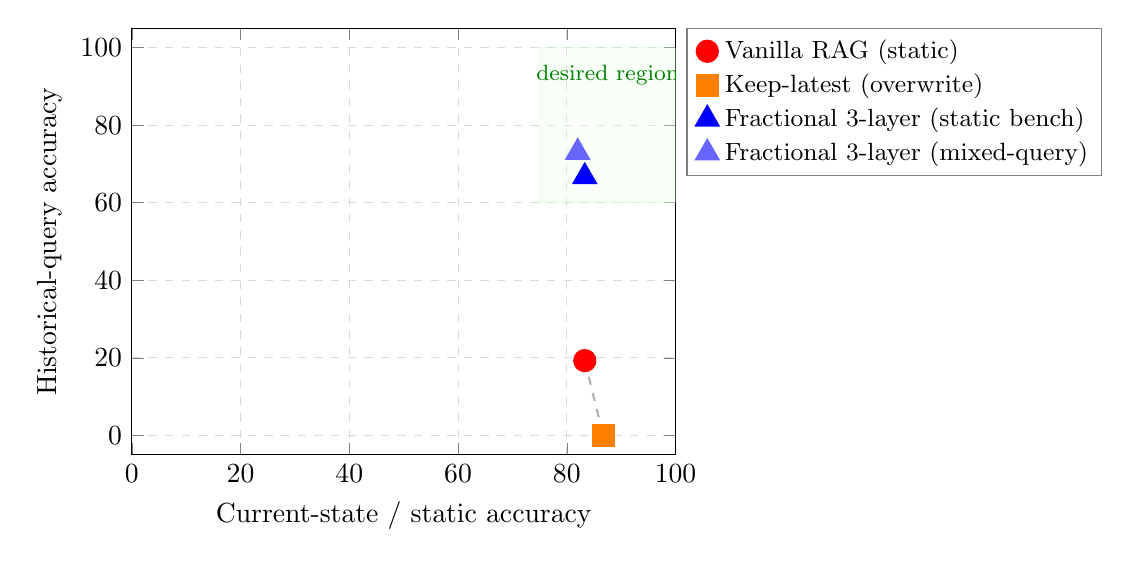
\begin{tikzpicture}
\begin{axis}[
    width=0.7\textwidth,
    height=7cm,
    xlabel={Current-state / static accuracy},
    ylabel={Historical-query accuracy},
    xmin=0, xmax=100,
    ymin=-5, ymax=105,
    xtick={0,20,40,60,80,100},
    ytick={0,20,40,60,80,100},
    legend style={
        at={(1.02,1)}, anchor=north west,
        fill=white, draw=black!50,
        font=\small,
    },
    legend cell align={left},
    grid=major,
    grid style={dashed, gray!30},
]
% Vanilla RAG: static 83.3, temporal 19.3 (from static benchmark)
\addplot[only marks, mark=*, mark size=4pt, red]
  coordinates {(83.3, 19.3)};
\addlegendentry{Vanilla RAG (static)}

% Keep-latest: static 86.7, temporal 75.4 (static benchmark)
% but mixed-query: current 47, historical 0
\addplot[only marks, mark=square*, mark size=4pt,
         orange]
  coordinates {(86.7, 0)};
\addlegendentry{Keep-latest (overwrite)}

% Fractional: static 83.3, temporal 66.7 (static)
% mixed-query: current ~82 overall-ish, historical 73
\addplot[only marks, mark=triangle*, mark size=5pt,
         blue]
  coordinates {(83.3, 66.7)};
\addlegendentry{Fractional 3-layer (static bench)}

\addplot[only marks, mark=triangle*, mark size=5pt,
         blue!60]
  coordinates {(82, 73)};
\addlegendentry{Fractional 3-layer (mixed-query)}

% Dashed frontier line through the baselines
\addplot[dashed, gray!60, thick] coordinates {
    (83.3, 19.3) (86.7, 0)
};

% Upper-right target region shading (informal)
\draw[green!30, fill=green!10, opacity=0.3]
  (axis cs: 75, 60) rectangle (axis cs: 100, 100);
\node[font=\footnotesize, green!50!black]
  at (axis cs: 87.5, 93) {desired region};

\end{axis}
\end{tikzpicture}
\caption{Pareto view of memory-architecture
tradeoffs.  Each marker is a system's pair of
accuracies on (current-state or static queries,
historical queries) under the same update stream.
Keep-latest maximizes current-state accuracy by
overwriting and scores $0\%$ on historical queries
by construction (it has deleted the relevant
facts).  Vanilla RAG retains history but cannot
separate current from historical values at
retrieval.  The fractional three-layer architecture
reaches the upper-right region neither baseline
can occupy: it retains old facts and answers
historical queries at $66$--$73\%$ while preserving
$82$--$83\%$ current-state accuracy.  The two blue
markers are the same system evaluated on two
different benchmarks
(\Cref{sec:static,sec:deployment}); the baselines
are shown only once each where the relevant
measurement exists.}
\label{fig:pareto}
\end{figure}

What the figure makes precise is architectural,
not just empirical.  \emph{Keep-latest cannot
answer historical queries.}  Not because of
parameter tuning or engineering: it has deleted the
relevant information.  \emph{Vanilla RAG cannot
answer current-state queries on a content-uniform
attribute.}  Not because of retrieval noise: the
embeddings are too similar to distinguish.  The
tradeoff is built into each baseline's policy.  The
three-layer architecture does not win by splitting
the difference; it wins by refusing the policy.
Facts are retained; temporal weighting at retrieval
time separates current from historical; the same
kernel evaluated at a different reference time
reconstructs past states
(\Cref{sec:deployment}).  The upper-right quadrant
is reachable because the architecture decouples
\emph{storage} (retain everything) from
\emph{scoring} (weight by age relative to the
query's reference time).

\begin{remark}[Scope of the Pareto result]
The figure plots two benchmarks and three system
configurations.  This is not a statement of
dominance against every possible memory
architecture---a carefully tuned hybrid store with
explicit version history and query routing could in
principle reach the same region, and learned
temporal kernels are an obvious direction we have
not explored.  What the figure shows is narrower:
the two natural baselines in
retrieval-augmented generation---overwriting and
uniform retention---each face a structural
ceiling, and the three-layer kernel-weighted
architecture reported here is the minimal
deviation that lifts both ceilings simultaneously.
\end{remark}


\section{Related Work}\label{sec:related}

\paragraph{Retrieval-augmented generation.}  RAG
systems~\cite{borgeaud2021retro,wu2022memorizing}
retrieve documents or tokens by embedding similarity
and condition the generation on them.  The present
system extends RAG with temporal structure in the
memory store and a routing mechanism to decide when
temporal weighting applies.

\paragraph{Continual and online learning.}
Parameter-efficient fine-tuning (LoRA, adapters)
modifies a small fraction of model weights to
incorporate new information.  The present system
modifies no weights; it achieves the key capability
typically used to motivate fine-tuning (incorporating
new information) through retrieval alone.

\paragraph{Temporal retrieval.}  Prior work on
time-aware retrieval typically uses exponential
decay~\cite{li2003time} or hand-tuned recency priors.
Using a fractional-calculus-derived kernel with
provable scale-invariance properties is, to our
knowledge, new in this application, though fractional
calculus has been used in other temporal-modeling
contexts.

\paragraph{Operator-theoretic foundations.}
Mittag-Leffler is the resolvent of the fractional
stochastic PDE
$\partial_t^\alpha m = -\lambda m + \mathrm{noise}$,
developed in \cite{fontes2026fracmem}.  Connection
to attention and the null-space problem it addresses
is developed in \cite{fontes2026opfac} and applied to
transformer architectures in \cite{fontes2026innov}.


\section{Limitations}\label{sec:limitations}

\paragraph{Benchmark scale.}  All experiments are at
store sizes of $\sim\!100$ to $\sim\!12{,}000$ facts.
Production memory systems may have millions of
entries.  Scaling requires approximate
nearest-neighbor methods (FAISS) and likely
category-aware retrieval; we have not tested these.

\paragraph{Normalization depends on templates.}
Current fact normalization uses hand-crafted templates
per category.  Production deployment would require
LLM-based extraction, which introduces errors not
measured here.

\paragraph{Routing is keyword-based.}  The $89\%$
temporal-query recall leaves $11\%$ of temporal
queries to be answered by pure cosine, where they
suffer the full temporal-disambiguation problem.  A
learned router or LLM-based routing would improve
coverage.

\paragraph{Simulated relevance in E1/E2.}  Our
mixed-rate benchmark uses a Gaussian noise model for
relevance rather than actual cosine similarity from
an embedding pipeline.  Design intent is to isolate
the kernel's contribution; a robustness check with
real embeddings is a natural next step.

\paragraph{Structural property is a kernel-level
result, not a system-level result.}
\Cref{thm:retention} bounds a quantity that depends
on the kernel alone.  \Cref{sec:when_kernel_secondary}
shows that this structural advantage does not
translate into system-level accuracy gains in every
regime.  The distinction is preserved throughout:
a kernel-asymptotic statement is separate from an
end-to-end benchmark result.


\section{Conclusion}\label{sec:conclusion}

A frozen language model with a three-layer memory
architecture adapts to new information in real time,
at $O(1)$ cost per entry, without modifying any
weights.  Architecture---normalize, route,
rerank---is the primary system-level contribution and
produces a $+27$~pp gain over vanilla retrieval-
augmented generation.

Mittag-Leffler's kernel, the resolvent of a
fractional stochastic PDE, has a structural retention
property that no exponential kernel can match: both
kernels have a fixed retention boundary $\tau^*$
(the maximum age at which a correct fact still
outranks a moderately-scored distractor), but
$\tau^*_{\mathrm{exp}}$ scales linearly in
$\lambda^{-1}$ while $\tau^*_{\mathrm{frac}}(\alpha,
\lambda)$ scales polynomially with exponent
$1/\alpha > 1$ and is unbounded as $\alpha \to 0$
(\Cref{thm:retention}).  The empirical results now
separate three claims.  First, in a broad synthetic
parameter-surface audit, fractional/Mittag-Leffler
reranking achieves the strongest best-tuned accuracy
($0.572$), and the result survives a dense $100$-point
EWMA audit ($0.495$).  Second, with real MiniLM
embeddings the sign survives: fractional reaches
$0.706$ versus $0.661$ for dense EWMA and finite
exponential mixtures and $0.646$ for power-law.  Third,
matched-scale controls show that the advantage is not
explained merely by longer memory: after matching EWMA
and power-law controls to the fractional half-life or
finite-horizon effective memory, the best matched
control reaches only $0.585$.

A structured frozen-decoder check adds a practical
adapter validation.  With a fixed local Ollama model,
fractional context selection reaches $0.970\pm0.017$
answer accuracy versus $0.778\pm0.048$ for dense EWMA
and $0.950\pm0.024$ for power-law.  This does not mean
the frozen model has learned internally.  The learning
state is external: the memory operator changes which
facts are supplied, and the fixed decoder extracts from
that context.

Stated precisely: architecture wins big, kernel wins
smaller but in a structurally grounded and empirically
surviving way, and the regimes where the kernel's
structural advantage translates into measurable accuracy
are a subset of the regimes where it is mathematically
superior.  The gap between these---what the kernel
provably does versus what a realistic retrieval system can
exploit---is itself a useful finding, and points to where
the next improvements in memory-augmented systems should
come from: better routing and candidate recall, not only
better temporal kernels.


\begin{thebibliography}{99}

\bibitem{borgeaud2021retro}
S.~Borgeaud et al., Improving language models by
retrieving from trillions of tokens,
arXiv:2112.04426, 2021.

\bibitem{wu2022memorizing}
Y.~Wu et al., Memorizing transformers,
arXiv:2203.08913, 2022.

\bibitem{li2003time}
X.~Li and W.~B.~Croft, Time-based language models,
\emph{CIKM}, 2003.

\bibitem{fontes2026opfac}
R.~Fontes, The operator derivative in continuous
stochastic calculus: a Hilbert energy space
framework, Quijotic Research, 2026.
Zenodo, \texttt{doi:10.5281/zenodo.18624822}.

\bibitem{fontes2026fracmem}
R.~Fontes, The fractional memory process:
well-posedness, spectral decomposition, and discrete
representation, Quijotic Research, 2026.
Preprint.

\bibitem{fontes2026innov}
R.~Fontes, Innovation attention: content-only
differencing for temporal reasoning in sequence
models, Quijotic Research, 2026.
Preprint.

\bibitem{gorenflo2014ml}
R.~Gorenflo, A.~A.~Kilbas, F.~Mainardi, and
S.~V.~Rogosin, \emph{Mittag-Leffler Functions,
Related Topics and Applications}, Springer
Monographs in Mathematics, Springer, 2014.

\bibitem{podlubny1999fractional}
I.~Podlubny, \emph{Fractional Differential
Equations}, Academic Press, 1999.

\bibitem{pollard1948ml}
H.~Pollard, The completely monotonic character of
the Mittag-Leffler function $E_a(-x)$,
\emph{Bulletin of the American Mathematical
Society} 54(12) (1948), 1115--1116.

\bibitem{wang2020minilm}
W.~Wang, F.~Wei, L.~Dong, H.~Bao, N.~Yang, and
M.~Zhou, MiniLM: Deep self-attention distillation
for task-agnostic compression of pre-trained
transformers, \emph{NeurIPS}, 2020.

\end{thebibliography}


\appendix

\section{Full Proof of
\texorpdfstring{\Cref{thm:retention}}{Theorem 5.1}}
\label{app:retention-proof}

We give the full argument promised by the sketch in
\Cref{sec:structural}.  Throughout, $\alpha \in (0,1)$,
$\lambda > 0$, and $r_c > r_d > 0$.  Recall the
retention boundary
\[
\tau^*(w) \;=\; \max \big\{ \tau \geq 1
  : r_c\,w(\tau) > r_d\,w(1) \big\},
\]
a real-valued constant that depends on $w$, $r_c$,
and $r_d$ but not on any external horizon.  For any
$T \geq 1$, $A(T) = \min(T, \lfloor\tau^*\rfloor)$.

\subsection*{Exponential case: \boldmath
$\tau^*_{\mathrm{exp}}(\lambda) = 1 +
\lambda^{-1} \ln(r_c/r_d)$\unboldmath}

For $w_{\mathrm{exp}}(t) = e^{-\lambda t}$, the
crossover condition $r_c w(\tau) > r_d w(1)$ is
\[
r_c e^{-\lambda \tau} > r_d e^{-\lambda}
\;\;\Longleftrightarrow\;\;
\lambda(\tau - 1) < \ln(r_c / r_d)
\;\;\Longleftrightarrow\;\;
\tau < 1 + \lambda^{-1}\ln(r_c/r_d).
\]
Equality at $\tau = \tau^*_{\mathrm{exp}}$ gives
\[
\tau^*_{\mathrm{exp}}(\lambda)
\;=\; 1 + \frac{1}{\lambda}\,\ln\!\frac{r_c}{r_d}.
\qquad\qed
\]

The boundary is linear in $\lambda^{-1}$ and
logarithmic in the content advantage $r_c/r_d$.  It
is strictly finite for every $\lambda > 0$.

\subsection*{Mittag-Leffler case: \boldmath
$\tau^*_{\mathrm{frac}}(\alpha, \lambda) =
\Theta(\lambda^{-1/\alpha})$\unboldmath{} and
unbounded as
\boldmath$\alpha \to 0$\unboldmath}

The Mittag-Leffler case requires the large-argument
asymptotic of $E_\alpha$ together with a monotonicity
statement that rules out $\tau^*_{\mathrm{frac}} =
\infty$.

\paragraph{Ingredient 1: Mittag-Leffler asymptotic.}
For $\alpha \in (0, 1)$, the Mittag-Leffler function
$E_\alpha(z) = \sum_{k=0}^{\infty}
z^k / \Gamma(\alpha k + 1)$ satisfies
\begin{equation}\label{eq:ml-asymptotic}
E_\alpha(-x) \;=\;
\frac{1}{x\,\Gamma(1-\alpha)}
\;+\; O(x^{-2})
\quad\text{as } x \to \infty,
\end{equation}
a classical result \cite{gorenflo2014ml,
podlubny1999fractional}.  In particular, there
exists $x_0 > 0$ and constants
$0 < c_1 < c_2$ such that
\begin{equation}\label{eq:ml-sandwich}
\frac{c_1}{x} \;\leq\;
E_\alpha(-x) \;\leq\;
\frac{c_2}{x}
\quad\text{for all } x \geq x_0.
\end{equation}

\paragraph{Ingredient 2: strict monotonicity and
finiteness of \boldmath$\tau^*_{\mathrm{frac}}$\unboldmath.}
By Pollard's representation \cite{pollard1948ml},
$E_\alpha(-x)$ for $\alpha \in (0,1)$ is completely
monotonic on $[0, \infty)$: it admits the integral
representation
\[
E_\alpha(-x) \;=\; \int_0^\infty e^{-xs}\,
M_\alpha(s)\,ds,
\]
where $M_\alpha$ is a non-negative probability
density on $(0, \infty)$.  Hence $E_\alpha(-x)$ is
strictly decreasing on $[0, \infty)$ from $E_\alpha(0)
= 1$ to $\lim_{x \to \infty} E_\alpha(-x) = 0$.
Therefore $w_{\mathrm{frac}}(\tau) = E_\alpha(
-\lambda \tau^\alpha)$ is strictly decreasing in
$\tau$ from $w_{\mathrm{frac}}(0) = 1$ to $0$.  The
set $\{\tau \geq 1 : r_c w_{\mathrm{frac}}(\tau) >
r_d w_{\mathrm{frac}}(1)\}$ is therefore an interval
$[1, \tau^*_{\mathrm{frac}})$ with $\tau^*_{\mathrm{frac}}
< \infty$, and $\tau^*_{\mathrm{frac}}$ is the unique
solution of
\begin{equation}\label{eq:tau-star-eqn}
r_c\,E_\alpha(-\lambda\,(\tau^*_{\mathrm{frac}})^\alpha)
\;=\; r_d\,E_\alpha(-\lambda).
\end{equation}

\paragraph{Leading-order asymptotic of
\boldmath$\tau^*_{\mathrm{frac}}$\unboldmath.}  When
$\lambda$ is small enough that $\lambda\,
(\tau^*_{\mathrm{frac}})^\alpha \geq x_0$, the
left-hand side of \eqref{eq:tau-star-eqn} is in the
asymptotic regime and, by \eqref{eq:ml-asymptotic},
\[
\frac{r_c}{\lambda\,(\tau^*_{\mathrm{frac}})^\alpha\,
  \Gamma(1-\alpha)}\,(1 + O(x_0^{-1}))
\;=\; r_d\,E_\alpha(-\lambda).
\]
Solving for $\tau^*_{\mathrm{frac}}$,
\begin{equation}\label{eq:tau-star-frac}
\tau^*_{\mathrm{frac}}(\alpha, \lambda)
\;=\; \Bigl(\frac{r_c}
  {r_d\,E_\alpha(-\lambda)\,\lambda\,
   \Gamma(1-\alpha)}\Bigr)^{1/\alpha}
\,(1 + o(1)),
\end{equation}
where the $o(1)$ error vanishes as $\lambda \to 0$
or as $\alpha \to 0$.

\paragraph{Two consequences.}
\textbf{(a)}  For fixed $\alpha \in (0,1)$,
$\tau^*_{\mathrm{frac}}(\alpha, \lambda)$ scales as
$\lambda^{-1/\alpha}$.  The exponent $1/\alpha > 1$
strictly exceeds the exponential kernel's exponent
$1$ on $\lambda^{-1}$, so for any fixed $\alpha$,
$\tau^*_{\mathrm{frac}}(\alpha, \lambda) /
\tau^*_{\mathrm{exp}}(\lambda) \to \infty$ as
$\lambda \to 0$.

\textbf{(b)}  For fixed $\lambda > 0$, sending $\alpha
\to 0$ makes the exponent $1/\alpha \to \infty$.
Provided the base of the exponent,
\[
\frac{r_c}{r_d\,E_\alpha(-\lambda)\,\lambda\,
  \Gamma(1-\alpha)},
\]
stays bounded away from $0$ (which it does: as
$\alpha \to 0$, $E_\alpha(-\lambda) \to 1/(1+\lambda)
> 0$ \cite{gorenflo2014ml} and $\Gamma(1-\alpha) \to
1$, so the base converges to $r_c(1+\lambda)/(r_d
\lambda) > 0$), the limit
\[
\lim_{\alpha \to 0^+} \tau^*_{\mathrm{frac}}(\alpha,
\lambda) \;=\; \infty.
\]
The retention boundary is therefore unbounded as a
function of $\alpha$.  \qed

\paragraph{Numerical check.}
At the tuning $\lambda = 0.05$, $r_c = 0.75$,
$r_d = 0.55$ used in \Cref{fig:retention}, the
closed-form asymptotic in \eqref{eq:tau-star-frac}
gives (before the $o(1)$ correction):
\[
\begin{array}{c|c|c}
\alpha & \tau^*_{\mathrm{frac}} \text{ from
  \eqref{eq:tau-star-frac}} &
  \text{numerical } \tau^*_{\mathrm{frac}} \\
\hline
0.3 & \approx 800 & 877 \\
0.2 & \approx 2 \times 10^4 & 31{,}040 \\
\end{array}
\]
The asymptotic formula agrees with direct numerical
evaluation of the bisection
$r_c\,E_\alpha(-\lambda\tau^\alpha) = r_d\,
E_\alpha(-\lambda)$ to leading order; the residual
gap is the $o(1)$ correction absorbed in the next
terms of \eqref{eq:ml-asymptotic}.  These numerical
values are the $\tau^*$ used to interpret
\Cref{fig:retention}: the saturation of the
$\alpha = 0.3$ curve between horizons $T = 1200$ and
$T = 2400$ is at $\min(T, \tau^*_{\mathrm{frac}})$ with
$\tau^*_{\mathrm{frac}} \approx 880$, and the
$\alpha = 0.2$ curve tracks the diagonal because
$\tau^*_{\mathrm{frac}} \approx 31{,}000$ exceeds every
plotted horizon.

\paragraph{Remark (what the theorem is not about).}
\Cref{thm:retention} is about the content-vs-recency
tradeoff: a single old-but-correct fact competing
against a single fresh-but-less-relevant distractor,
in deterministic arithmetic.  It is not about the
following distinct kernel property, which surfaces
elsewhere in the fractional-memory literature and is
worth separating:

\emph{Monotone-order preservation through
floating-point underflow.}  In tasks where multiple
candidates have identical content scores and the
retriever must recover a consistent ordering of them
by age alone, exponential weights at large ages can
underflow to literal float64 zero across all
candidates, collapsing the ranking to random
tiebreaking.  Mittag-Leffler weights, bounded below
by \eqref{eq:ml-sandwich}, remain in representable
range much further out.  This is a numerical
property of the functional form, not a statement
about $\tau^*$, and does not bear on
\Cref{thm:retention}.  Downstream applications that
rely on this second property (e.g., long-context
needle-in-haystack benchmarks where all candidate
chunks share content match score) are governed by
the underflow threshold of the chosen representation,
not by the retention boundary.


\end{document}
